\documentclass{article}
\usepackage[UTF8]{ctex}

\usepackage{amsmath}        %数学公式
\usepackage{amssymb}
\usepackage{cases}          %联立编号
\usepackage{cite}           %引用

\usepackage{graphicx}       %插入图片
\usepackage{float}          %设置图片浮动位置
\usepackage{subfigure}      %插入多图时用子图显示

\usepackage{listings}
\usepackage{xcolor}

\usepackage{anyfontsize}    %解决一个奇怪的字体大小报错问题
\usepackage{fancyhdr}       %页眉、页脚、页码
\usepackage[a4paper, margin=1in]{geometry}    %纸张大小
\usepackage{longtable}

\title{\bf\huge 概率论与数理统计 - 作业 2}
\author{Jerry}
\date{\today}

\lstset{
    basicstyle          =   \sffamily,          % 基本代码风格
    keywordstyle        =   \bfseries,          % 关键字风格
    commentstyle        =   \rmfamily\itshape,  % 注释的风格,斜体
    stringstyle         =   \ttfamily,  % 字符串风格
    flexiblecolumns,                % 别问为什么,加上这个
    numbers             =   left,   % 行号的位置在左边
    showspaces          =   false,  % 是否显示空格,显示了有点乱,所以不现实了
    numberstyle         =   \zihao{-5}\ttfamily,    % 行号的样式,小五号,tt等宽字体
    showstringspaces    =   false,
    captionpos          =   t,      % 这段代码的名字所呈现的位置,t指的是top上面
    frame               =   lrtb,   % 显示边框
}

\lstdefinestyle{Python}{
    language        =   Python, % 语言选Python
    basicstyle      =   \zihao{-5}\ttfamily,
    numberstyle     =   \zihao{-5}\ttfamily,
    keywordstyle    =   \color{blue},
    keywordstyle    =   [2] \color{teal},
    stringstyle     =   \color{magenta},
    commentstyle    =   \color{red}\ttfamily,
    breaklines      =   true,   % 自动换行,建议不要写太长的行
    columns         =   fixed,  % 如果不加这一句,字间距就不固定,很丑,必须加
    basewidth       =   0.5em,
}

\begin{document}
\maketitle

\section*{T1. }

$P(A+B+C)=P(A+(B+C))=P(A)+P(B+C)-P(A(B+C))=P(A)+P(B)+P(C)-P(BC)-P(A(B+C))$

$P(A(B+C))=P(AB+AC)=P(AB)+P(AC)-P((AB)(AC))=P(AB)+P(AC)-P(ABC)$

$\therefore P(A+B+C)=P(A)+P(B)+P(C)-P(BC)-P(A(B+C))=P(A)+P(B)+P(C)-P(BC)-P(AB)-P(AC)+P(ABC)$

\section*{T2. }

(a. )$0 \leq P(·|B) \leq 1$

~

$P(·|B)=\dfrac{P(·B)}{P(B)}\leq \dfrac{P(B)}{P(B)}=1$

$P(·|B)=\dfrac{P(·B)}{P(B)}\geq 0$

~

(b. )$P(\Omega)=1,P(\phi)=0$

~

$P(·|B)$在$B\subset ·$时,即$B \cap · =B$时,有$P(·|B)=\dfrac{P(·B)}{P(B)}=\dfrac{P(B)}{P(B)}=1$

$P(·|B)$在$B\subset ·$时,即$B \cap · =\phi$时,有$P(·|B)=\dfrac{P(·B)}{P(B)}=\dfrac{\phi}{P(B)}=0$

~

(c. )加法公理

~

$P(A_1|B)+P(A_2|B)+...+P(A_n|B)=\dfrac{P(A_1B)}{P(B)}+\dfrac{P(A_2B)}{P(B)}+\dfrac{P(A_3B)}{P(B)}+...+\dfrac{P(A_nB)}{P(B)}$

$=\dfrac{P(A_1B)+P(A_2B)+...+P(A_nB)}{P(B)}=\dfrac{P((A_1+A_2+...+A_n)B)}{P(B)}$,($A_1,A_2,...,A_n$互斥)

$=P((A_1+A_2+A_3+...+A_n)|B)$

\section*{T3. }

(a. )$P(A) \geq P(A|B)$

-- 不正确

当$P(B)<1$时,令$A=B$,$P(A|B)=P(B|B)=1$,$P(A)=P(B)<P(A|B)$

(b. )不存在既互斥也相互独立的事件$A$,$B$

-- 不正确

互斥满足$P(A)+P(B)=1$,$P(AB)=0$,独立要求$P(AB)=P(A)P(B)$,若考虑$P(A)=1$,$P(B)=0$,则有事件$A$、$B$互相独立且互斥。

(c. )*若$P(ABC)=P(A)P(B)P(C)$,则$A$,$B$,$C$独立。

-- 不正确

若$P(C)=0$,则无论$A$、$B$关系均有$P(ABC)=P(A)P(B)P(C)=0$,不能保证$A$、$B$互斥。

\section*{T4. }

掷两个骰子,枚举所有可能情况,我们可以得到掷骰子得到2\~{}12的概率分别为

\begin{table}[!ht]
    \centering
    \begin{tabular}{|l|l|l|l|l|l|l|l|l|l|l|l|}
    \hline
        点数 & 2 & 3 & 4 & 5 & 6 & 7 & 8 & 9 & 10 & 11 & 12 \\ \hline
        概率 & 1/36 & 2/36 & 3/36 & 4/36 & 5/36 & 6/36 & 5/36 & 4/36 & 3/36 & 2/36 & 1/36 \\ \hline
    \end{tabular}
\end{table}

(a. )$A_2\&A_3$

~

$P(A_2)=\dfrac{1+3+5+5+3+1}{36}=\dfrac{18}{36}$,$P(A_3)=\dfrac{2+5+4+1}{36}=\dfrac{12}{36}$

~

$P(A_2A_3)=\dfrac{5+1}{36}=\dfrac{6}{36}$

~

$\because P(A_2)P(A_3)=P(A_2A_3)$

$\therefore A_2$与$A_3$互相独立

(b. )$A_2\&A_5$

~

$P(A_2)=\dfrac{1+3+5+5+3+1}{36}=\dfrac{18}{36}$,$P(A_5)=\dfrac{4+3}{36}=\dfrac{7}{36}$

~

$P(A_2A_5)=\dfrac{3}{36}$

~

$\because P(A_2)P(A_5)\neq P(A_2A_5)$

$\therefore A_2$与$A_5$不互相独立

\section*{T5. }

(a. )条件独立不意味着独立

考虑一个正四面体骰子,四个面分别为1,2,3,4

事件$A$:掷出的数为1

事件$B$:掷出的数为1或2

事件$C$:掷出的数为1或2

~

则有$P(A)=\dfrac{1}{4}$,$P(B)=\dfrac{1}{2}$,$P(A|C)=\dfrac{1}{2}$,$P(B|C)=1$,$P(AB)=\dfrac{1}{4}$,$P(AB|C)=\dfrac{1}{2}$

~

此时,满足条件独立:$P(AB|C)=P(A|C)P(B|C)$,但不满足独立$P(AB)\neq P(A)P(B)$

(b. )独立不意味着条件独立

考虑一个正四面体骰子,四个面分别为1,2,3,4

事件$A$:掷出的数为1或2

事件$B$:掷出的数为1或3

事件$C$:掷出的数为1或2或3

~

则有$P(A)=\dfrac{1}{2}$,$P(B)=\dfrac{1}{2}$,$P(A|C)=\dfrac{1}{3}$,$P(B|C)=\dfrac{1}{3}$,$P(AB)=\dfrac{1}{4}$,$P(AB|C)=\dfrac{1}{3}$

~

此时,满足独立:$P(AB)=P(A)P(B)$,但不满足条件独立$P(AB|C)\neq P(A|C)P(B|C)$

\section*{T6. }

我们可以认为每次$A$是否发生为一个独立的事件,记$n$次重复,$A$始终不发生为事件$T$,第$n$次重复$A$不发生事件为$T_n$

$P(T)=P(T_1T_2T_3...T_n)=P(T_1)P(T_2)P(T_3)...P(T_n)=(1-\varepsilon)^n$

$\because 0<\epsilon<1$

$\therefore 0<1-\epsilon<1$

$\therefore \lim_{n \to \infty}(1-\varepsilon)^n=0$

$\therefore P(T)=0$,即$A$迟早不发生的概率为0,$A$迟早要发生的概率为1

\section*{T7. }

定义事件$A$为翻出红色,事件$B$为翻出黑色,则事件$AB$为拿到一面红色一面黑色的卡,概率为$\frac{1}{3}$

$P(B|A)=P(BA)\div P(A)=\frac{1}{3}\div\frac{2}{3}=\frac{1}{2}$

\section*{T8. }

公平,理由如下:

(1. )在此方法下,每人抽到的概率显然为$\frac{1}{n}$

(2. )在此方法下,我们假设第$i$个人没有抽中,对第$i+1$个人考虑

定义事件“在第i人轮次,此人未抽中”为事件$N_i$,“在第i人轮次,此人抽中”为事件$Y_i$

定义事件“第i人未结束”为事件$Continue_i$,“第i人结束”为事件$End_i$

第$i+1$人抽中的概率为$P(End_{i+1})=P(Continue_i)P(Y_{i+1})$

$P(Continue_i)=P(Continue_{i-1})P(N_i)=P(N_i)P(N_{i-1})...P(N_2)P(N_1)$

$=\frac{n-1}{n}\frac{n-2}{n-1}...\frac{n-i}{n-i+1}=\frac{n-i}{n}$

$P(Y_{i+1})=\frac{1}{n-i}$

$P(End_{i+1})=P(Continue_i)P(Y_{i+1})=\frac{1}{n-i}\frac{n-i}{n}=\frac{1}{n}$

(2. )的中签概率与(1. )中的结果相同,故两种方式是公平的

\section*{T9. }

记患病为事件$A$,阳性为事件$B$,有以下公式可计算出检验阳性下患病的概率

~

$P(A|B)=\dfrac{P(AB)}{P(B)}=\dfrac{0.6 \times 1}{0.6 \times 1+0.4 \times 0.3}=\dfrac{0.6}{0.72}=83.33\%$

~

概率大于80$\%$,故应建议病人做手术

\section*{T10. }

(1. )

设拥有$k$元时,输光离场的概率为$p_k$,在第一次参与后有$p$的概率变成$k+1$元,
有$1-p$的概率变成$k-1$元,可以推出$$p_k=pp_{k+1}+(1-p)p_{k-1}$$

对这个式子处理得到$$(1-p)(p_k-p_{k-1})=p(p_{k+1}-p_k)$$

从而$$\frac{p_{k+1}-p_k}{p_k-p_{k-1}}=\frac{1-p}{p}$$

得到$$\frac{p_n-p_{n-1}}{p_1-p_0}=(\frac{1-p}{p})^{n-1}$$

相加,得到$$p_n-p_0=(p_n-p_{n-1})+(p_{n-1}-p_{n-2})+...+(p_1-p_0)$$

$$p_n-p_0=(p_1-p_0)((\frac{1-p}{p})^{n-1}+(\frac{1-p}{p})^{n-2}+...+(\frac{1-p}{p})^{0})$$

(1.a. )$p\neq0.5$

$$p_n-p_0=(p_1-p_0)(\frac{1-(\frac{1-p}{p})^n}{1-\frac{1-p}{p}})$$

$$p_k-p_0=(p_1-p_0)(\frac{1-(\frac{1-p}{p})^k}{1-\frac{1-p}{p}})$$

两式相除,得到$$\frac{p_n-p_0}{p_k-p_0}=\frac{1-(\frac{1-p}{p})^n}{1-(\frac{1-p}{p})^k}$$

考虑到$p_{n}=0,p_0=1$,故$$p_k=1-\frac{1-(\frac{1-p}{p})^k}{1-(\frac{1-p}{p})^n}$$

(1.b. )$p=0.5$

$$p_n-p_0=n(p_1-p_0)$$

$$p_k-p_0=k(p_1-p_0)$$

两式相除,得到$$\frac{p_n-p_0}{p_k-p_0}=\frac{n}{k}$$

考虑到$p_{n}=0,p_0=1$,故$$p_k=1-\frac{k}{n}$$

(2. )

在$p\leq0.5$时,

(2.a. )$p<0.5$

$$\lim_{n\to\infty}p_k=1-\lim_{n\to\infty}\frac{1-(\frac{1-p}{p})^k}{1-(\frac{1-p}{p})^n}=1-0=1$$

(2.b. )$p=0.5$

$$\lim_{n\to\infty}p_k=1-\lim_{n\to\infty}\frac{k}{n}=1-0=1$$

\section*{T11. }

假设有$n$个个体,计算下一时刻这个物种数量的数学期望。
该物种分裂、消亡、不变的概率均为$\frac{1}{3}$,$E(n)=\frac{1}{3}n\cdot 2+\frac{1}{3}n\cdot 1+\frac{1}{3}n\cdot 0=n$,为一个恒定值。

我们假设最终灭亡的概率为$p$,在有$n$个个体时的灭亡概率为$p_n$,则$$p_1=\frac{1}{3}p_0+\frac{1}{3}p_1+\frac{1}{3}p_2$$

考虑到$n$个生物灭亡的概率就是全部相乘,即$p_n=p_1^n$,$p_0=1$,有$$p_1=\frac{1}{3}+\frac{1}{3}p_1+\frac{1}{3}p_1^2$$

解方程得$$p=1$$

即该生物灭亡的概率为100\%

\section*{T12. }

使用甲药治好疾病的概率$P(M)=0.8\times0.8+0.1\times0.05+0.1\times0.1=0.655$

使用乙药治好疾病的概率$P(N)=0.8\times0.6+0.1\times0.9+0.1\times0.9=0.66$

乙药治好病的概率更大,故应使用乙药来治疗。

考虑甲药与乙药的概率几乎相同,且甲药能以最大的概率治好最可能患的病,也可以采用。

\section*{T13. }

(1. )

$P(B_1)=\frac{1}{2}\cdot\frac{4}{5}+\frac{1}{2}\cdot\frac{2}{5}=\frac{3}{5}$,
$P(U_1|B_1)=\frac{P(U_1B_1)}{B_1}=\frac{\frac{4}{10}}{\frac{3}{5}}=\frac{2}{3}$,
$P(U_1)=\frac{1}{2}$

$P(U_1|B_1)>P(U_1)$,第一次摸出黑球说明这个袋子更可能是$U_1$而非$U_2$

(2. )

当放回后,我们可以认为第二次摸球与第一次情况相同,从而$P(B_2)=P(B_1)=\frac{2}{3}$。

当不放回时,$P(B_2)=\frac{1}{2}\cdot (\frac{1}{2}\cdot (\frac{4}{5}\cdot\frac{3}{4}+\frac{3}{5}\cdot\frac{3}{4}) + \frac{1}{2}\cdot (\frac{2}{5}\cdot\frac{1}{4}+\frac{3}{5}\cdot\frac{3}{4}))=\frac{2}{5}$。
此时,$P(B_2)$与$P(B_1)$不同的原因是第一次的摸球对第二次的摸球产生了干扰。

(3. )

当不放回时,$P(B_2|B_1)=\frac{2}{3}\cdot\frac{3}{4}+\frac{1}{3}\cdot\frac{1}{4}=\frac{7}{12}$。
此时,$P(B_2)$与$P(B_1)$不同的原因是第一次的摸球的颜色对袋子的分布产生了干扰。

(4. )

假设拿的袋子为$U_1$,第$n+1$次取出黑球的概率为$\frac{4}{5}$;假设拿的袋子为$U_2$,第$n+1$次取出黑球的概率为$\frac{2}{5}$。
由此可见仅需考虑前$n$次抓取对袋子的分布产生的干扰即可。

计算前$n$次均取出黑球时,拿到的袋子为$U_1$的概率:

~

$P_{nU_1}=\dfrac{(\frac{4}{5})^n}{(\frac{4}{5})^n+(\frac{2}{5})^n}=\dfrac{1}{1+(\frac{2}{5}\cdot\frac{5}{4})^n}=\dfrac{1}{1+(\frac{1}{2})^n}$

~

故下一次抓出黑球的概率$P(B_{n+1}|B_1B_2...B_n)=\frac{4}{5}P_{nU_1}+\frac{2}{5}P_{nU_2}$

~

$=\dfrac{4}{5}\cdot\dfrac{1}{1+(\frac{1}{2})^n}+\dfrac{2}{5}\cdot\dfrac{(\frac{1}{2})^n}{1+(\frac{1}{2})^n}
=\dfrac{4+2\cdot(\frac{1}{2})^n}{5\cdot(1+(\frac{1}{2})^n)}=\dfrac{4\cdot 2^n+2}{5\cdot 2^n+5}$

~

进一步令$n \to \infty$,这个概率的极限是$\frac{4}{5}$,直观理解为前$n$次抽球均为黑球说明黑球说明这个袋子更可能是黑球多的那一个,
而下一次为一次新的随机抽取过程,可以理解为在$U_1$袋子再次随机抽取,从而抽出黑球的概率为$\frac{4}{5}$

(5. )

由(4. )可得,

进一步令$P_{nU_1}$的$n \to \infty$,这个概率的极限是$1$,这说明无限次抽取均为黑球说明这个袋子更可能是黑球多的那一个。

\section*{T14. }

(1. )

必定获胜的策略:假设在甲处投$x$元,则在乙处投$100-x$元,甲胜利的概率为$p$,期望收益$W=p\cdot 5x+(1-p)\cdot \frac{5}{2}(100-x)-100=7.5px-250p-2.5x+150$,
其中$p$为参数,$x$为我控制的变量。对$W$求导,可以得出$x=\frac{100}{3}$时,$W$有最值,此时无论胜负如何都能得到$W=\frac{200}{3}$

(2. )

$W_1=25P_1+0(1-P_1)-5=0$,$W_2=25P_1+0(1-P_1)-10=0$

在甲的眼中$B$队的获胜概率$P_1=20\%$,在乙的眼中$A$队的获胜概率$P_2=40\%$

$P_1+P_2=60\%<1$,这也就是(1. )中存在必定获利策略的原因

\section*{T15. }

(1. )

其中,x轴为实验次数,y轴为相对频率

\begin{center}
    \begin{figure}[H] %H为当前位置,!htb为忽略美学标准,htbp为浮动图形
        \centering %图片居中
        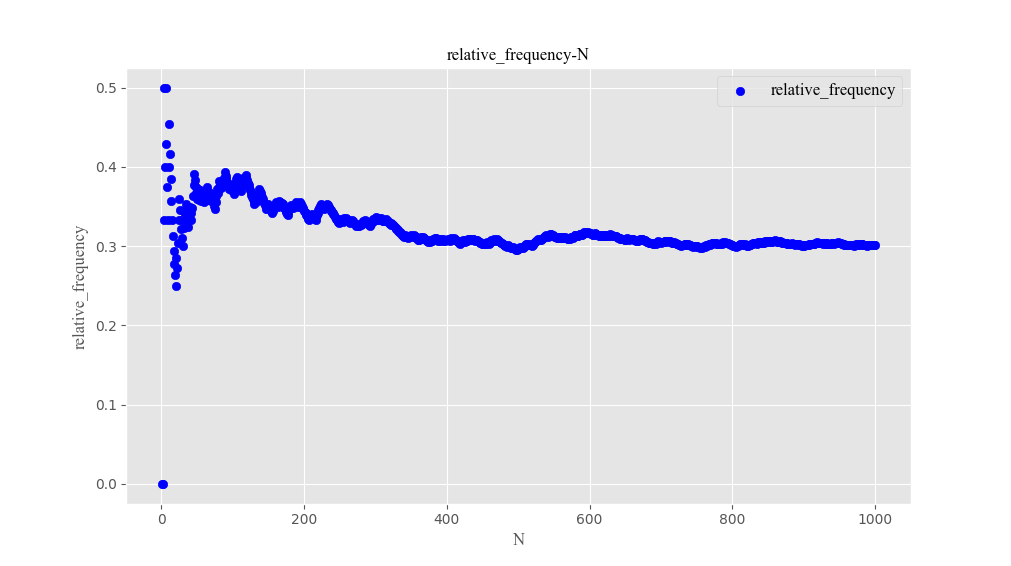
\includegraphics[width=1.0\textwidth]{img/Figure_1.png} %插入图片,[]中设置图片大小,{}中是图片文件名
        \caption{RelativeFrequency-N} %最终文档中希望显示的图片标题
        \label{fig1} %用于文内引用的标签
    \end{figure}
\end{center}

源代码如下:

\lstinputlisting[
    style       =   Python,
    caption     =   {\bf simulation1.py},
    label       =   {1}
]{code/simulation1.py}

(2. )

其中,x轴为实验次数,y轴为正面向上的次数之和

\begin{center}
    \begin{figure}[H] %H为当前位置,!htb为忽略美学标准,htbp为浮动图形
        \centering %图片居中
        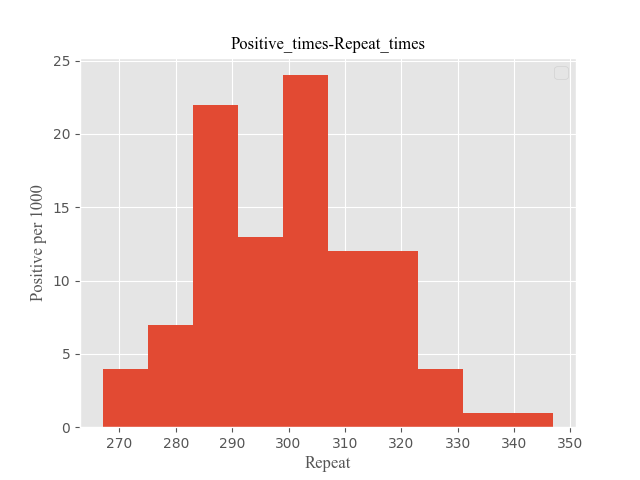
\includegraphics[width=0.6\textwidth]{img/Figure_2.png} %插入图片,[]中设置图片大小,{}中是图片文件名
        \caption{?} %最终文档中希望显示的图片标题
        \label{fig2} %用于文内引用的标签
    \end{figure}
\end{center}

源代码如下:

\lstinputlisting[
    style       =   Python,
    caption     =   {\bf simulation2.py},
    label       =   {2}
]{code/simulation2.py}

(3. )

上述 100 次试验正面朝上次数的平均值为299.41,$np$为300,偏差不超过0.5\%

源代码如下:

\lstinputlisting[
    style       =   Python,
    caption     =   {\bf simulation3.py},
    label       =   {3}
]{code/simulation3.py}

(4. )

改变simulation*.py中的p/n/repeat即可

\end{document}